
\subsection{Mathmatical Model of a single Perceptron}	
		
A perceptron is nothing more than a function that takes in several inputs and produces an output of either 0 or 1.\\ \\
The input of perceptron is usually modeled as a column vector. Let $X(n\times1)$ represent this column vector. The perceptron applies weights to each values in the $X$ and then sums them together. In other words, the perceptron finds a linear combination of the matrix $X$ as show below.
$$
X = 
\begin{bmatrix}
	x_1 \\
	x_2 \\
	x_3 \\
	\vdots \\
	x_n
\end{bmatrix} 
$$
Let $\alpha$ be a possible linear combination of $X$. 
$$
	\alpha = \sum_{i=1}^{n} a_ix_i = a_1x_1 + a_2x_2 + \dots + a_nx_n
$$
At first all $a_i$ are chosen randomly, however, during the training process they will get adjusted until they are able to produce the optimal output. The training process we utilized in out program is called back propagation and will be covered later in this paper.\\

The next step of the perceptron utilizes an activation function. An activation function can be either 0 or 1, depending on a threshold value. The threshold value is selected based on the specific use of the perceptron. Below is an example of an activation function. Let $T$ represent the threshold value.

$$f(x) = 
	\begin{array}{cc}
  	\{ & 
    \begin{array}{cc}
    	1 & x >= T \\
    	0 & x < T
    \end{array}
\end{array}
$$

The output of the perceptron is the output of the activation function above.

\subsection{Layering perceptrons}

Perceptrons gain a lot more functionality when they are used in combination with other perceptrons. Let $p_i$ represent a perceptron. Perceptrons are stack together to build column vectors of perceptrons as show below.

$$
	P = \begin{bmatrix}
		p_1 \\
		p_2 \\
		\vdots \\
		p_3
	\end{bmatrix}
$$

A column vector of perceptrons is called a layer. There are three kinds of perceptron layers. There is an input layer. The input layer is always the first layer in any multilayered perceptron. There is the output layer. This layer is always the last layer, and as the name suggests this is the output of the multilayer perceptron. In between the output layer and the input layer are the hidden layers. There can be any number of hidden layers in a perceptron. Each of these layers use the output of the layer right before it as their input.

\begin{center}
	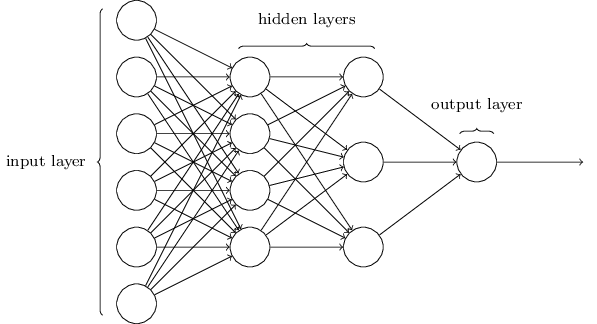
\includegraphics[scale=0.5]{multilayer-perceptron2}
\end{center}

The diagram aboves represents how a multilayer perceptron is structured. Notice how each perceptron takes in all the outputs from the layer before it. This multilayer perceptron only has 1 output, however, it is possible to structure a perceptron to output multiple values if needed. An example of a multilayer perceptron with multiple outputs is shown below.

\begin{center}
	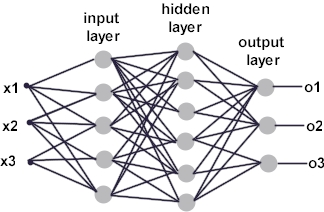
\includegraphics[scale=0.5]{multilayer-perceptron}
\end{center}

The structure above is used when the problem is more complex. For example, a perceptron that takes in the pixel values of an image of a hand written number and then outputs what it thinks the number is needs 10 outputs, 1 for each possible value. \\

A perceptron can be a very useful tool for difficult problems such as recognizing handwriting, because they can be used to build any possible logical function. However, designing multilayered perceptron to read handwriting is significantly easier than trying to write the explicit logical statements for it.

\subsection{Training}

The most important part of any perceptron is to train it so that it produces the output that is expected of it. The training process is simply changing the weights applied in each perceptron in each layer until it produces the optimal outcome. This is accomplished using training data, data which the result is already known. In the hand drawing example used before, the training data would be images that have been tagged 